% ============================================================
%  Appendix for \ourbench
%  \input{} this file after \appendix in main.tex
%  Requires: booktabs, tabularx, enumitem packages
% ============================================================

% ---- Appendix Table of Contents ----
% \clearpage
% \begin{center}
%   {\LARGE\bfseries Appendices}
% \end{center}
% \vspace{2em}

% \newcommand{\appdots}{\hspace{0.3em}\leaders\hbox{\normalfont.}\hfill\hspace{0.3em}}

% \setlength{\parindent}{0pt}
% {\setlength{\parskip}{7pt}
% \textbf{\large A}\quad{\large\bfseries Benchmark Comparison Dimensions\appdots\pageref{app:benchmark_dims}}

% \textbf{\large B}\quad{\large\bfseries Character Construction and Memory Pipeline\appdots\pageref{app:character}}

% \hspace{2em}B.1\enspace Profile Specification\appdots\pageref{app:stage_a}

% \hspace{2em}B.2\enspace Memory Quota Allocation\appdots\pageref{app:stage_b}

% \hspace{2em}B.3\enspace Memory Generation Protocol\appdots\pageref{app:stage_c}

% \hspace{2em}B.4\enspace Quality Audit and Repair\appdots\pageref{app:stage_d}

% \hspace{2em}B.5\enspace Memory Schema\appdots\pageref{app:schema}

% \hspace{2em}B.6\enspace Dataset Statistics\appdots\pageref{app:stats}

% \textbf{\large C}\quad{\large\bfseries Scenario Construction and Validation\appdots\pageref{app:scenario}}

% \hspace{2em}C.1\enspace Scenario Schema and Example\appdots\pageref{app:scenario_schema}

% \hspace{2em}C.2\enspace Validation Protocol and Coverage\appdots\pageref{app:scenario_validation}

% \textbf{\large D}\quad{\large\bfseries Evaluation Instance Construction\appdots\pageref{app:eval_instance}}

% \hspace{2em}D.1\enspace Automated Annotation Pipeline\appdots\pageref{app:annotation}

% \hspace{2em}D.2\enspace Expert Validation Protocol\appdots\pageref{app:annotation_protocol}

% \hspace{2em}D.3\enspace MCQ Assembly\appdots\pageref{app:mcq_assembly}

% \hspace{2em}D.4\enspace Analysis of an Example\appdots\pageref{app:case_study}

% \textbf{\large E}\quad{\large\bfseries Model--Model Agreement Analysis\appdots\pageref{app:model_agreement}}

% \textbf{\large F}\quad{\large\bfseries Limitations and Future Works\appdots\pageref{app:limitations}}

% \textbf{\large G}\quad{\large\bfseries Prompts\appdots\pageref{app:prompts}}

% \hspace{2em}G.1\enspace Character Generation Prompt\appdots\pageref{app:prompt_character}

% \hspace{2em}G.2\enspace Memory Generation Prompt\appdots\pageref{app:prompt_memory}

% \hspace{2em}G.3\enspace Scenario Expansion Prompt\appdots\pageref{app:prompt_scenario}

% \hspace{2em}G.4\enspace Annotation Prompts\appdots\pageref{app:prompt_annotation}
% }

% \clearpage

% ============================================================
\section{Benchmark Comparison Dimensions}
\label{app:benchmark_dims}
% ============================================================

Table~\ref{tab:benchmark_comparison} in the main text compares \ourbench with related benchmarks across six dimensions. We define each dimension below. These six dimensions are not intended to exhaust all possible aspects of human-like agent evaluation. Instead, they operationalize the minimum design requirements for the construct targeted in this work: psychologically grounded, scenario-level behavioural decision-making.

\begin{itemize}[leftmargin=1.5em, itemsep=4pt]
  \item \textbf{Big-Five grounded.} The benchmark explicitly adopts the Big Five (OCEAN) personality framework as the basis for character or persona design---not merely mentioning personality, but operationalising it via structured trait dimensions.

  \item \textbf{Lifespan coverage.} The benchmark covers multiple developmental life stages (e.g., childhood, adolescence, adulthood) grounded in developmental psychology theory (e.g., Erikson, Levinson). Multi-session dialogue time spans that simulate passage of time without reference to developmental stage do not qualify.

  \item \textbf{Episodic memory.} The benchmark includes or evaluates structured autobiographical/episodic memory content---first-person narratives encoding what happened, how it felt, and how it shaped the agent---rather than mere interaction logs or fact stores.

  \item \textbf{Scenario eval.} Evaluation requires an agent to make a concrete behavioural decision within a structured situational context. Pure factual recall, question-answering, or stylistic consistency checks do not qualify.

  \item \textbf{Expert annot.} The benchmark's gold labels or quality judgments involve domain experts (e.g., psychologists, clinical researchers) as primary annotators or validators---not crowd workers or automated scoring alone.

  \item \textbf{Trait-driven decision.} Evaluation specifically tests whether behavioural decisions are grounded in and consistent with the character's personality profile. Benchmarks that only test whether the agent recalls the right facts or matches a surface stylistic pattern do not qualify.
\end{itemize}

% ============================================================
\section{Character Construction and Memory Pipeline}
\label{app:character}
% ============================================================

This appendix details the four-stage pipeline used to construct the 11 character profiles and their 11{,}000 long-horizon memories, the unified memory schema, and the resulting dataset statistics. The pipeline structure and its connection to the benchmark are described in the main text (\S\ref{sec:character}); here we report the implementation details and quantitative artefacts omitted for brevity.

% ---- A.1 Profile Specification ----
\subsection{Profile Specification}
\label{app:stage_a}

Each of the 11 character profiles is stored as a JSON object in \texttt{characters\_phase11.json}. Beyond the Big Five vector and archetype label reported in Table~\ref{tab:characters}, each profile contains:

\begin{itemize}[leftmargin=1.5em, itemsep=2pt]
  \item \textbf{Self-value logic} (1 sentence): the character's core cognitive operating principle, derived from the dominant trait.
  \item \textbf{Core behavioural patterns} (8 items): fixed trait expressions that must appear across all generated memories.
  \item \textbf{Occupation rationale}: the occupation is chosen to be consistent with the dominant trait so that work-domain memories are ecologically valid.
\end{itemize}

Table~\ref{tab:persona} provides the self-value logic and three representative core behavioural patterns for each character. Full 8-pattern lists are stored in \texttt{characters\_phase11.json}.

\begin{table}[h]
\centering
\caption{The 11 character archetypes. Bolded scores mark the defining extreme dimension; CHAR\_11 is the all-neutral baseline.}
\label{tab:characters}
\small
\begin{tabular}{llcccccl}
\toprule
\textbf{ID} & \textbf{Archetype} &
\textbf{O} & \textbf{C} & \textbf{E} & \textbf{A} & \textbf{N} &
\textbf{Occupation} \\
\midrule
CHAR\_01 & N-High  & .85 & .50 & .30 & .55 & \textbf{.95} & Freelance content creator \\
CHAR\_02 & N-Low   & .50 & .55 & .50 & .60 & \textbf{.10} & Community GP \\
CHAR\_03 & C-High  & .45 & \textbf{.95} & .40 & .60 & .30 & Project manager \\
CHAR\_04 & C-Low   & .80 & \textbf{.10} & .60 & .65 & .45 & Freelance programmer \\
CHAR\_05 & E-High  & .65 & .55 & \textbf{.95} & .70 & .35 & Sales director \\
CHAR\_06 & E-Low   & .75 & .70 & \textbf{.10} & .45 & .50 & Indie game developer \\
CHAR\_07 & A-High  & .55 & .60 & .55 & \textbf{.95} & .55 & Non-profit coordinator \\
CHAR\_08 & A-Low   & .65 & .85 & .45 & \textbf{.10} & .35 & Startup co-founder \\
CHAR\_09 & O-High  & \textbf{.95} & .35 & .65 & .55 & .40 & Anthropology lecturer \\
CHAR\_10 & O-Low   & \textbf{.10} & .75 & .40 & .55 & .45 & Building-materials retailer \\
CHAR\_11 & Neutral & .50 & .50 & .50 & .50 & .50 & Local journalist \\
\bottomrule
\end{tabular}
\end{table}
\begin{table}[h]
\centering
\caption{The 11 character archetypes. Bolded scores mark the defining extreme dimension; CHAR\_11 is the all-neutral baseline.}
\label{tab:characters}
\small
\begin{tabular}{llcccccl}
\toprule
\textbf{ID} & \textbf{Archetype} &
\textbf{O} & \textbf{C} & \textbf{E} & \textbf{A} & \textbf{N} &
\textbf{Occupation} \\
\midrule
CHAR\_01 & N-High  & .85 & .50 & .30 & .55 & \textbf{.95} & Freelance content creator \\
CHAR\_02 & N-Low   & .50 & .55 & .50 & .60 & \textbf{.10} & Community GP \\
CHAR\_03 & C-High  & .45 & \textbf{.95} & .40 & .60 & .30 & Project manager \\
CHAR\_04 & C-Low   & .80 & \textbf{.10} & .60 & .65 & .45 & Freelance programmer \\
CHAR\_05 & E-High  & .65 & .55 & \textbf{.95} & .70 & .35 & Sales director \\
CHAR\_06 & E-Low   & .75 & .70 & \textbf{.10} & .45 & .50 & Indie game developer \\
CHAR\_07 & A-High  & .55 & .60 & .55 & \textbf{.95} & .55 & Non-profit coordinator \\
CHAR\_08 & A-Low   & .65 & .85 & .45 & \textbf{.10} & .35 & Startup co-founder \\
CHAR\_09 & O-High  & \textbf{.95} & .35 & .65 & .55 & .40 & Anthropology lecturer \\
CHAR\_10 & O-Low   & \textbf{.10} & .75 & .40 & .55 & .45 & Building-materials retailer \\
CHAR\_11 & Neutral & .50 & .50 & .50 & .50 & .50 & Local journalist \\
\bottomrule
\end{tabular}
\end{table} 

\begin{table}[h]
\centering
\caption{Character persona specifications: self-value logic and representative behavioural patterns.}
\label{tab:persona}
\small
\resizebox{\textwidth}{!}{%
\begin{tabular}{p{1.5cm}p{4.2cm}p{8.5cm}}
\toprule
\textbf{ID} & \textbf{Self-Value Logic} & \textbf{Representative Core Patterns (of 8)} \\
\midrule
CHAR\_01 \newline N-High &
Pre-emptive self-attack is the primary defence against anticipated rejection. &
Catastrophising minor setbacks; ruminating on past mistakes; over-interpreting social micro-expressions. \\
\midrule
CHAR\_02 \newline N-Low &
Evidence over emotion; unverified information is not a basis for action; ambiguity is waste, not threat. &
Maintaining equanimity under pressure; fact-seeking before reacting; emotional containment in conflict. \\
\midrule
CHAR\_03 \newline C-High &
Only controllable and verifiable systems are trustworthy; any deviation signals danger. &
Exhaustive checklists; pre-task risk scanning; micro-managing format details even under low stakes. \\
\midrule
CHAR\_04 \newline C-Low &
The flow state is the only thing worth pursuing; plans are others' games; deadlines are external noise. &
Abandoning tasks mid-way; chasing novelty over completion; losing focus outside deep-work states. \\
\midrule
CHAR\_05 \newline E-High &
A room is an opportunity; silence is waste; converting strangers into relationships is the primary metric. &
Initiating social contact within minutes; thinking aloud by default; reading silence as a buying signal. \\
\midrule
CHAR\_06 \newline E-Low &
Social interaction is costly and modelled as threat; deep work requires full solitude. &
Treating each social event as a drain needing recovery; preferring async communication; refusing open-plan settings. \\
\midrule
CHAR\_07 \newline A-High &
Conflict harms everyone; every person has goodwill if given the right frame. &
Seeking the mediating position in disputes; over-attributing benign intent; postponing direct refusals. \\
\midrule
CHAR\_08 \newline A-Low &
Every interaction has a power structure; cost-benefit drives all decisions; sentiment is not data. &
Mapping authority hierarchies immediately; treating conflict as information; direct assertion without packaging. \\
\midrule
CHAR\_09 \newline O-High &
Every ``obvious'' belief is worth questioning; fixed thinking is the primary enemy. &
Deep-diving any novel idea encountered; redesigning routines into new habits; sustaining flow in creative immersion. \\
\midrule
CHAR\_10 \newline O-Low &
Proven methods are crystallised wisdom; change and novelty are costs, not opportunities. &
Defending stable suppliers and routines; distrusting ``innovation'' discourse; valuing what works over what is new. \\
\midrule
CHAR\_11 \newline Neutral &
Balance and moderation across all dimensions; no single trait dominates decision-making. &
Context-sensitive responses; moderate engagement across social and task domains; avoiding extremes. \\
\bottomrule
\end{tabular}%
}
\end{table}

% ---- A.2 Memory Quota Allocation ----
\subsection{Memory Quota Allocation}
\label{app:stage_b}

The 45-year span (ages 6--50) is divided into 45 one-year segments. For a character that already has $k$ memories, the algorithm computes the deficit $d = 1{,}000 - k$ and distributes it proportionally across segments according to a weight vector $\mathbf{w}$ defined by developmental salience:

\begin{equation}
  q_t = \left\lfloor d \cdot \frac{w_t}{\sum_j w_j} \right\rfloor + \epsilon_t
\end{equation}

where $q_t$ is the quota for segment $t$, $w_t$ is higher for transitional stages (Adolescence, Early Adult Transition, Age-30 Transition), and $\epsilon_t \in \{0,1\}$ is a rounding correction to ensure $\sum_t q_t = d$ exactly. The resulting distribution concentrates memories in formative periods, consistent with empirical findings on self-defining memory clustering \cite{singer1995seeing}.

% ---- A.3 Memory Generation Protocol ----
\subsection{Memory Generation Protocol}
\label{app:stage_c}

Memories are generated using Claude Sonnet 4.6 via the Anthropic Messages API. Each batch covers a 2--5 year age window and targets 45--50 memories. The structured system prompt injects three constraint layers:

\begin{enumerate}[leftmargin=1.5em, itemsep=2pt]
  \item \textbf{Character constraints}: full Big Five vector, occupation, self-value logic, and all eight core behavioural patterns from Appendix~\ref{app:stage_a}.
  \item \textbf{Developmental context}: target age window, life-stage label, and the core developmental task from Table~\ref{tab:stage_dist} (Appendix~\ref{app:stats}).
  \item \textbf{Rubin coverage}: per-dimension guidance requiring organic integration of all five dimensions without explicit section labels.
  Unlike semantic memory---which stores abstract, decontextualized facts (e.g., ``failed a job interview'')---each \texttt{content\_full} narrative must encode information that collectively reconstructs the subjective texture of the experience and is irreducible to propositional fact-storage.
  The five dimensions are:
  \begin{enumerate}[leftmargin=1.5em, itemsep=1pt]
    \item \textit{Sensory detail}—concrete sights, sounds, smells, or tactile cues that bind the memory to a specific time and place, supplying the perceptual specificity that distinguishes an episode from a generic category;
    \item \textit{Dialogue reconstruction}—verbatim or near-verbatim exchange that encodes interpersonal dynamics and relational positioning; a semantic summary such as ``argued with a superior'' erases the tone, phrasing, and the character's reactive stance that carry personality-relevant information;
    \item \textit{Inner monologue}—in-the-moment appraisals and automatic thoughts that directly express the character's trait vector $\mathbf{p}_i$ (e.g., catastrophising for high-$N$); collapsing this to a single emotion label, as semantic memory does, discards the cognitive signature of the trait;
    \item \textit{Somatic response}—physiological arousal signals (heart rate, muscle tension, nausea) that capture affective intensity as embodied knowledge inaccessible to propositional fact-stores and that resist post-hoc rationalisation;
    \item \textit{Aftermath}—psychological consequences within one week that trace schema-level impact beyond the immediate event, encoding how the episode altered the character's beliefs or coping patterns rather than merely recording its outcome.
  \end{enumerate}
\end{enumerate}

To prevent within-batch duplication, the prompt seeds topic diversity across five scenario domains: workplace, interpersonal, health, creative, and daily life. All batches for all 11 characters are generated in parallel, each writing to an independent file (\texttt{\_charXX\_bYY.txt}) for fault-tolerant incremental collection.

\paragraph{Structured output format.}
Each memory is delimited by a unique header (\texttt{===MEM\_XX\_NNN===}) followed by a two-part block: a metadata preamble in \texttt{key: value} format, and a narrative body separated by a \texttt{---content\_full---} delimiter. This deterministic text format avoids bracket-level JSON formatting errors common in large-scale LLM structured output.

\begin{table}[h]
\centering
\caption{Memory schema field specification. \textbf{S} = Structural (core identity and narrative fields); \textbf{R} = Retrieval-index (fields used for memory activation and search); \textbf{P} = Psychological annotation (fields encoding personality and affect).}
\label{tab:schema}
\small
\setlength{\tabcolsep}{5pt}
\renewcommand{\arraystretch}{1.25}
\begin{tabular}{>{\bfseries}cp{2.8cm}p{3.2cm}p{6.0cm}}
\toprule
\textbf{Role} & \textbf{Field} & \textbf{Constraint} & \textbf{Description} \\
\midrule
\rowcolor{blue!8}
S & id               & \textit{MEM\_XX\_NNN}          & Unique identifier encoding character and sequence number. \\
\rowcolor{blue!8}
S & timeline         & \textit{stage label (age)}     & Life-stage tag from Table~\ref{tab:stage_dist}. \\
\rowcolor{blue!8}
S & context          & \textit{15--30 chars}          & Compact situational setting (where / when). \\
\rowcolor{blue!8}
S & content\_summary & \textit{20--40 chars}          & One-sentence event gist; used for fast retrieval pre-filtering. \\
\rowcolor{blue!8}
S & content\_full    & \textit{2{,}000--4{,}500 chars}    & First-person narrative embedding all five Rubin dimensions. \\
\midrule
\rowcolor{green!8}
R & triggers         & \textit{4 keywords}            & Cue words that activate this memory during simulation. \\
\rowcolor{green!8}
R & relevance\_tags  & \textit{4 tags}                & Thematic tags linking memory to life threads and EMS clusters. \\
\midrule
\rowcolor{orange!8}
P & psych\_conclusion  & \textit{1 sentence}          & Long-term psychological interpretation of the event. \\
\rowcolor{orange!8}
P & behavior\_policy   & \textit{1 sentence}          & Implicit behavioural rule reinforced by this memory~\cite{young2006schema}. \\
\rowcolor{orange!8}
P & emotion\_signature & \textit{\{primary, secondary,}        & Affective signature supporting mood-congruent retrieval~\cite{bower1981}; \\
\rowcolor{orange!8}
  &                    & \textit{\quad intensity $\in [0,1]$\}} & intensity amplified for high-N characters. \\
\bottomrule
\end{tabular}
\end{table}


% ---- A.4 Quality Audit and Repair ----
\subsection{Quality Audit and Repair}
\label{app:stage_d}

The audit step screens each memory against the following six defect criteria, implemented via a combination of regex patterns and LLM-based classifiers (e.g., \texttt{audit\_god\_view.py}). Any failure routes the memory to the targeted repair loop.

\begin{enumerate}[leftmargin=1.5em, itemsep=4pt]
  \item \textbf{Perspective Drift (Omniscient Narrator).} Violating the first-person narrative constraint. Detected when the narrator uses post-hoc knowledge or future-tense markers (e.g., ``years later,'' ``I didn't know then''). This violates the strict ``in-the-moment'' constraint.

  \item \textbf{Perspective Drift (Adult Evaluation).} Specifically flags child-age memories ($\leq 12$) that use adult-level cognitive appraisals or retrospective phrases (e.g., ``looking back,'' ``I now understand'').

  \item \textbf{Field-Length Inversion.} \texttt{context} exceeding 60 characters or \texttt{content\_summary} exceeding 100 characters, indicating narrative leakage into metadata fields.

  \item \textbf{Semantic Duplication.} Redundant life episodes within the same developmental age window. This is detected using a cosine similarity threshold of $> 0.85$ over TF-IDF vector representations of the narratives; 

  \item \textbf{Length Violation.} \texttt{content\_full} below 2{,}000 characters (insufficient Rubin coverage) or above 4{,}500 characters (excessive verbosity).

  \item \textbf{Schema-Vocabulary Inflation.} Use of high-register psychoanalytic terms (e.g., ``abandonment schema'', ``dysregulation'') in low-intensity episodes ($< 0.4$), indicating over-psychologisation.
\end{enumerate}

\paragraph{Repair procedure.}
Flagged memories enter a targeted repair loop: only the defective field(s) are regenerated using an issue-specific instruction appended to the original generation prompt. For example, a perspective-drift failure supplies the original \texttt{context} and \texttt{content\_summary} and instructs the model to rewrite \texttt{content\_full} from a strict first-person viewpoint. Up to three repair attempts are made per defect; memories still non-compliant after three attempts are logged for manual review. The repaired dataset is saved incrementally every five fixes to prevent data loss.

% ---- A.5 Memory Schema ----
\subsection{Memory Schema}
\label{app:schema}

Table~\ref{tab:schema} specifies all ten fields of the unified memory schema. Fields are grouped by functional role: structural (S), retrieval-index (R), and psychological annotation (P).


% ---- A.6 Dataset Statistics ----
\subsection{Dataset Statistics}
\label{app:stats}

\paragraph{Per-character statistics.}
Table~\ref{tab:dataset_stats} reports the finalised per-character memory counts, average \texttt{content\_full} lengths, and mean emotion intensities. All 11 characters achieved the target of exactly 1{,}000 memories. The mean narrative length across the corpus is 3{,}307.2 characters, and the mean emotion intensity is 0.620, with N-High (CHAR\_01) predictably exhibiting the highest intensity (0.697) and N-Low (CHAR\_02) the lowest (0.499).

\begin{table}[h]
\centering
\caption{Per-character dataset statistics.}
\label{tab:dataset_stats}
\small
\begin{tabular}{llccc}
\toprule
\textbf{ID} & \textbf{Archetype} & \textbf{Memories} & \textbf{Avg.\ Length (chars)} & \textbf{Avg.\ Intensity} \\
\midrule
CHAR\_01 & N-High   & 1,000 & 2856.6 & 0.697 \\
CHAR\_02 & N-Low    & 1,000 & 3374.9 & 0.499 \\
CHAR\_03 & C-High   & 1,000 & 3497.3 & 0.640 \\
CHAR\_04 & C-Low    & 1,000 & 2927.0 & 0.652 \\
CHAR\_05 & E-High   & 1,000 & 3519.4 & 0.659 \\
CHAR\_06 & E-Low    & 1,000 & 3326.2 & 0.625 \\
CHAR\_07 & A-High   & 1,000 & 3445.8 & 0.621 \\
CHAR\_08 & A-Low    & 1,000 & 2939.0 & 0.598 \\
CHAR\_09 & O-High   & 1,000 & 3485.6 & 0.659 \\
CHAR\_10 & O-Low    & 1,000 & 3540.6 & 0.612 \\
CHAR\_11 & Neutral  & 1,000 & 3405.8 & 0.561 \\
\midrule
\textbf{Total / Mean} & --- & \textbf{11,000} & \textbf{3307.2} & \textbf{0.620} \\
\bottomrule
\end{tabular}
\end{table}

\paragraph{Life-stage distribution.}
Table~\ref{tab:stage_dist} reports the aggregate memory distribution across developmental stages (pooled over all 11 characters). Higher density in School age and Adolescence (combined 32.8\%) and in the early-career stages (Early adult trans.\ + Entering adult world, 25.2\%) reflects the weighted quota scheme in Appendix~\ref{app:stage_b} and is consistent with the empirical distribution of self-defining memories across the lifespan \cite{singer1995seeing}.

\begin{table}[h]
\centering
\caption{Aggregate memory distribution across life stages (all 11 characters, $N=11{,}000$).}
\label{tab:stage_dist}
\small
\begin{tabular}{lrr}
\toprule
\textbf{Stage} & \textbf{Count} & \textbf{Proportion} \\
\midrule
School age (6--12)              & 1,812 & 16.5\% \\
Adolescence (13--18)            & 1,793 & 16.3\% \\
Early adult trans.\ (19--22)   & 1,286 & 11.7\% \\
Entering adult world (23--27)  & 1,489 & 13.5\% \\
Age-30 transition (28--32)     & 1,380 & 12.5\% \\
Settling down (33--40)         & 1,805 & 16.4\% \\
Midlife transition (41--45)    &   795 &  7.2\% \\
Entering midlife (46--50)      &   640 &  5.8\% \\
\midrule
\textbf{Total} & \textbf{11,000} & \textbf{100\%} \\
\bottomrule
\end{tabular}
\end{table}

\label{app:trait_value_dist}


% ============================================================
\section{Scenario Construction and Validation}
\label{app:scenario}
% ============================================================

This appendix documents the schema, coverage validation, and an end-to-end example of the 64 character-agnostic scenarios constructed in \S\ref{sec:scenario}.

% ---- B.1 Schema and Example ----
\subsection{Scenario Schema and Example}
\label{app:scenario_schema}

Table~\ref{tab:scenario_components} details the four-component schema used by the LLM-assisted expansion stage (\S\ref{sec:scenario}, Stage~2). The schema enforces a uniform structure across all 64 scenarios so that downstream evaluation, retrieval, and ground-truth annotation can rely on stable field semantics. The system prompt that drives the expansion---including the field-level constraints, the character-agnostic principles, and the controlled vocabularies for Big Five and Schwartz keys---is reproduced in Appendix~\ref{app:prompt_scenario}.

\begin{table}[h]
\centering
\caption{Four-component schema for scenario expansion with detailed descriptions.}
\label{tab:scenario_components}
\setlength{\tabcolsep}{2.5pt}
\small
\begin{tabularx}{\textwidth}{p{2.8cm}p{3.1cm}X}
\toprule
\textbf{Component} & \textbf{Purpose} & \textbf{Content Description} \\
\midrule
Metadata & Anchoring \& summary & id, name, description, life stage, age, intensity level \\
\midrule
Environmental Setting & Contextual atmosphere & Physical location, specific time, emotional/social atmosphere \\
\midrule
Narrative Context & Background establishment & Detailed situational buildup, prior events, social dynamics, character relationships \\
\midrule
Trigger Event & Decision catalyst & Specific sender, verbatim dialogue/message content that requires immediate response \\
\bottomrule
\end{tabularx}
\end{table}

The following example illustrates a fully expanded scenario instance under this schema. It demonstrates how abstract attributes such as developmental stage, DIAMONDS dimension, and contextual narrative are instantiated into a concrete social situation involving high-stakes decision making, while strictly maintaining the character-agnostic constraint.
\label{app:ExampleofScenario}

\begin{tcolorbox}[
  breakable,
  colback=blue!5,
  colframe=blue!60!black,
  title={\textbf{Scenario Instance}},
  fonttitle=\bfseries,
  rounded corners,
  boxrule=1.0pt
]
\begin{Verbatim}[fontsize=\scriptsize, breaklines=true, breaksymbolleft={}, breaksymbolright={}, breakindent=1em]
{
  "id": "SCN_SCHOOL_AGE_3",
  "stage": "school_age",
  "age_range": "6-11 years",
  "age": 10,
  "diamonds_dimension": "Adversity",
  "name": "The Shattered Group Presentation",
  "category": "Integrity Dilemma / Responsibility Crisis",
  "intensity": "High",
  "description_for_agent": "A high-pressure adversity scenario involving a teammate's failure, loss of a core project artifact, and an imminent public presentation requiring a moral decision.",
  "setting": {
    "location": "Elementary school multipurpose auditorium backstage waiting area",
    "time": "09:45 AM",
    "atmosphere": "Noisy, tense, and suffocating"
  },
  "context_text": "Today is the school's annual \"Final Innovation Showcase Competition\". Students, homeroom teachers, the dean of studies, the principal, and a dense crowd of parents are seated in the auditorium. The air conditioning seems to be broken, making the space stiflingly hot. Your five-person group was randomly assigned by the teacher, but over the past two weeks, almost all research, writing, and rehearsal work has been completed by you alone. The only delegated task - transporting your group's \"solar system model\" built from cardboard, clay, and LED lights - was assigned to a group member who lives nearby, just two bus stops away. Backstage, harsh fluorescent lights illuminate the waiting area. You can hear the previous group presenting \"Plant Respiration\", occasionally interrupted by low questions from judges. The host has just announced: \"Next group, please get ready.\" You turn toward the entrance - the teammate responsible for the model has not yet arrived.",
  "trigger_event": {
    "sender": "Responsible group member",
    "message_content": "(bursts in through the side entrance of the backstage area, sweating heavily, school uniform collar crooked, hands empty, eyes red) I... I left the model on the bus! I only noticed after getting off... I ran after it for two stops but couldn't catch it... (voice trembling, nearly crying) Please don't tell the teacher it was me, okay? My mom is sitting in the third row today. She just punished me last week for losing things... If she finds out, she will beat me again... Let's just tell the teacher that the model was accidentally damaged by the cleaning staff last night, okay? Without the model, we can just talk through it and get by... (before finishing, the homeroom teacher steps in from behind the curtain holding a scoring sheet, brows furrowed, scanning the empty hands) \"Where is your model? You go on stage in 30 seconds - where is it?\""
  }
}
\end{Verbatim}
\end{tcolorbox}

% ---- B.2 Validation protocol and coverage ----
\subsection{Validation Protocol and Coverage}
\label{app:scenario_validation}

The Stage-3 expert validation in \S\ref{sec:scenario} ensures that the generated scenarios are individually plausible and \emph{collectively well-structured}---spanning the psychological situation space rather than concentrating on a narrow slice of it. The validation proceeds in two passes:

\begin{enumerate}[leftmargin=1.5em, itemsep=2pt]
  \item \textbf{Logical and psychological screening.} Two doctoral-level psychology researchers jointly check each scenario for logical consistency and psychological plausibility. Any flagged scenario is revised by consensus before entering the second pass.
  \item \textbf{Independent rating and conflict resolution.} Both reviewers independently rate each scenario on the eight DIAMONDS dimensions (1--7 Likert) and identify the scenario's dominant Schwartz value-conflict pair. Disagreements above 1 point trigger joint re-assessment.
\end{enumerate}

We do not require a uniform DIAMONDS rating distribution; the goal is that each dimension be exercised across both ends of its intensity range, so that no situational characteristic is structurally absent. Reviewers also confirm that the central tension of each scenario corresponds to a theoretically opposing Schwartz value pair on the circumplex, rather than an incidental disagreement.

\paragraph{DIAMONDS coverage.}
\label{app:diamonds_coverage}
The DIAMONDS framework characterizes situations along eight psychologically grounded dimensions: \textit{Duty}, \textit{Intellect}, \textit{Adversity}, \textit{Mating}, \textit{pOsitivity}, \textit{Negativity}, \textit{Deception}, and \textit{Sociality}. These dimensions capture recurring situational affordances relevant to human behavior and decision-making.

Table~\ref{tab:diamonds_distribution} reports, for each DIAMONDS dimension, the empirical distribution of expert ratings across the 64 scenarios. Coverage is intentionally non-uniform to reflect ecological prevalence: \textit{Mating} and \textit{Positivity} concentrate at low ratings (most scenarios are not romantic or unambiguously positive), while \textit{Negativity} concentrates at high ratings (the benchmark is built around psychologically demanding situations).


\begin{table}[h]
\centering
\caption{Distribution of expert DIAMONDS ratings across the 64 scenarios. Each row sums to 64.}
\label{tab:diamonds_distribution}
\small
\begin{tabular}{lccccccc}
\toprule
\textbf{DIAMONDS}
& \textbf{1} & \textbf{2} & \textbf{3}
& \textbf{4} & \textbf{5}
& \textbf{6} & \textbf{7} \\
\midrule
Duty        & 10 & 10 & 10 & 5  & 11 & 8  & 10 \\
Intellect   & 4  & 7  & 11 & 21 & 10 & 5  & 6  \\
Adversity   & 6  & 7  & 9  & 6  & 14 & 7  & 15 \\
Mating      & 48 & 8  & 0  & 1  & 0  & 1  & 6  \\
Positivity  & 34 & 15 & 5  & 6  & 2  & 2  & 0  \\
Negativity  & 0  & 1  & 0  & 1  & 11 & 12 & 39 \\
Deception   & 5  & 12 & 9  & 10 & 6  & 8  & 14 \\
Sociality   & 5  & 6  & 10 & 14 & 14 & 11 & 4  \\
\bottomrule
\end{tabular}
\end{table}

\paragraph{Schwartz value-conflict coverage.}
\label{app:schwartz_coverage}
Table~\ref{tab:schwartz_pairs} lists the most frequent Schwartz value-conflict pairs implicitly embedded in the 64 scenarios, as identified by expert annotators. The dominant axes are \textit{Self-Direction} versus \textit{Conformity/Security}, which together account for nearly half of all annotated conflicts and reflect the autonomy--obligation tension that underlies most adult moral dilemmas.

\begin{table}[h]
\centering
\caption{Top-10 Schwartz value-conflict pairs across the 64 scenarios.}
\label{tab:schwartz_pairs}
\small
\begin{tabular}{clc}
\toprule
\textbf{Rank} & \textbf{Value-conflict pair} & \textbf{Count} \\
\midrule
1  & Conformity vs Self-Direction   & 17 \\
2  & Security vs Self-Direction     & 12 \\
3  & Benevolence vs Security        & 11 \\
4  & Achievement vs Conformity      & 6  \\
4  & Benevolence vs Self-Direction  & 6  \\
4  & Benevolence vs Universalism    & 6  \\
7  & Achievement vs Benevolence     & 5  \\
7  & Benevolence vs Hedonism        & 5  \\
7  & Power vs Universalism          & 5  \\
10 & Conformity vs Security         & 3  \\
\bottomrule
\end{tabular}
\end{table}


% ============================================================
\section{Evaluation Instance Construction}
\label{app:eval_instance}
% ============================================================

This appendix details how character--scenario pairs are instantiated into the final 673 multiple-choice questions, including the automated annotation pipeline, the expert validation protocol, and the test-instance assembly.

\subsection{Automated Annotation Pipeline}
\label{app:annotation}

The automated annotation pipeline (\S\ref{sec:CreatingEvaluationInstances}, Stage~1) produces a single candidate \textit{final decision} for every (character, scenario) pair via two coordinated LLM stages. The full system prompts driving each stage are reproduced in Appendix~\ref{app:prompt_annotation}.

\paragraph{Memory activation (coarse-to-fine retrieval).} For every (character, scenario) pair we retrieve the episodic memories most likely to enter the character's working memory in that situation. A coarse pass with \textit{Claude-Haiku-4.5} screens the character's full $1{,}000$-memory pool for relevance and yields roughly $75$--$125$ candidates per scenario (Stage~1 prompt; see Appendix~\ref{app:prompt_activation}). A fine pass with \textit{Claude-Sonnet-4.6} then globally re-ranks the candidates and retains the top $50$ memories (Stage~2 prompt; see Appendix~\ref{app:prompt_finalize}). The two-stage design preserves recall during screening and concentrates expensive reasoning on the smaller, harder ranking decision.

\paragraph{Response generation.} Conditioned jointly on the character's full personality profile (Big Five traits, Schwartz value orientations, and self-narrative) and the top-$50$ activated memories, \textit{Claude-Sonnet-4.6} role-plays the character in first person and produces the structured Ground Truth annotation (Stage~3 prompt; see Appendix~\ref{app:prompt_gt}). The annotation contains a stream-of-consciousness inner trace and the two-sentence \textit{final decision} that defines the gold label.

\begin{tcolorbox}[
  breakable,
  colback=blue!5,
  colframe=blue!60!black,
  title={\textbf{Example of Ground Truth Annotation}},
  fonttitle=\bfseries,
  rounded corners,
  boxrule=1.0pt
]
\begin{Verbatim}[fontsize=\scriptsize, breaklines=true, breaksymbolleft={}, breaksymbolright={}, breakindent=1em]
{
  "SCN_ENTERING_MIDLIFE_5": {
    "character_id": "CHAR_04_C_LOW",
    "scenario_id": "SCN_ENTERING_MIDLIFE_5",
    "final_decision": "I choose to break the silence and step into this unfamiliar emptiness together with her, instead of retreating into familiar routines. I stand up, smile, and say: \"Lets go-lets head out. Doesnt matter where, we will just go.\""
  }
}
\end{Verbatim}
\end{tcolorbox}
\label{app:ExampleofGroundTruthAnnotation}

\subsection{Expert Validation Protocol}
\label{app:annotation_protocol}

The Stage-2 expert validation in \S\ref{sec:CreatingEvaluationInstances} engages a four-expert team with a consensus-then-arbitration rule. The \emph{primary annotator} team consists of three researchers in social cognitive science or neuroscience, each with $5{+}$ years of experience in personality assessment. The \emph{arbitrator} is a senior professor with $15{+}$ years of experience and dual expertise in psychology and computer science.

\paragraph{Suitability check.} For each (character, scenario) pair, every primary annotator first decides whether the pair is fundamentally suitable for evaluation. If any annotator identifies an irreconcilable conflict between the character's profile and the scenario, the entire pair is discarded.

\paragraph{Independent review.} For each surviving pair, the three primary annotators independently review the LLM-produced annotation and rate it on a three-tier scale:
\begin{enumerate}[leftmargin=1.5em, itemsep=2pt]
  \item \textit{Acceptable as-is.}
  \item \textit{Acceptable with modifications.} The reviewer writes out the required revisions.
  \item \textit{Unacceptable.}
\end{enumerate}
The review focuses on the \textit{final decision} field and asks whether it is psychologically plausible and consistent with the character's established personality profile.

\paragraph{Consensus-then-arbitration.} If all three primary annotators rate the annotation as \textit{acceptable as-is}, it is adopted directly as the gold annotation. Otherwise the case is escalated to the arbitrator, who reviews the annotation together with each primary annotator's rating and written rationale, and either edits the annotation or rewrites it from scratch. If the arbitrator deems the case fundamentally unfit, the (character, scenario) pair is discarded.

\paragraph{Outcome.} In total, $31$ (character, scenario) pairs were discarded across the suitability and arbitration steps, leaving $673$ expert-validated gold annotations. Over half of all surviving cases were unanimously rated \textit{acceptable as-is} and passed directly without arbitration, and the per-token edit rate of expert revisions over the LLM-generated annotation content was approximately $15\%$, evidence that the LLM-generated annotations are already of high quality before expert refinement.

\subsection{MCQ Assembly}
\label{app:mcq_assembly}

The Stage-3 test-instance assembly in \S\ref{sec:CreatingEvaluationInstances} converts each expert-validated annotation into a four-option multiple-choice question. For a given scenario the target character's validated response serves as the correct option; the ten validated responses of the remaining ten characters to the \emph{same} scenario form the candidate distractor pool. Because every MCQ has only three distractor slots, we ask \textit{Claude-Sonnet-4.6} to pick three out of ten such that the resulting question is neither trivial nor ambiguous, applying two filters:
\begin{itemize}[leftmargin=1.5em, itemsep=2pt]
  \item \textbf{Similarity filter.} A candidate that is semantically too close to the target option is rejected, since it would make the question ambiguous (multiple plausibly correct answers).
  \item \textbf{Relevance filter.} A candidate whose content is obviously off-scenario is rejected, since it would make the correct option trivially identifiable by elimination.
\end{itemize}
The selected three distractors and the target-character option are then randomly shuffled before being written out, removing positional and ordering bias from the final benchmark. The procedure yields exactly one MCQ per surviving annotation, for a total of 673 instances.


% ============================================================
\subsection{Analysis of an Example from \ourbench}
\label{app:case_study}
% ============================================================
Figure~\ref{fig:case_study} presents a representative MCQ from \ourbench, drawn from the \emph{settling\_down} life stage (ages 33--40) under the ``community injustice'' scenario. All four options revolve around the same surface-level action---\emph{filing an individually-named complaint to the housing bureau}---but are generated under distinct character profiles with different Big Five configurations. Only option B uniquely corresponds to the target character CHAR\_06, an independent game developer characterized by very low Extraversion (0.10) and high Conscientiousness (0.70). This design deliberately decouples \textbf{surface behavior} from \textbf{personality-driven pragmatic expression}, requiring the model to reason over each character's internal logic rather than rely on superficial action matching.

The correct answer B exhibits three tightly coupled personality signals of CHAR\_06. First, the statement ``the materials are already prepared'' is not an improvised claim but a retrospective reframing of a previously completed decision, reflecting a work style grounded in solitary preparation and consistent execution (``well-prepared, follows through''). Second, ``I won't push for joint signatures; I'll go on my own'' contrasts sharply with the cooperative stance in option A (CHAR\_02), which reflects coalition-building behavior (e.g., ``if you're willing to help find materials, I'll take it''). In contrast, B contains no recruitment, coordination, or affective engagement, consistent with a ``polite-but-distant'' interaction style and a preference for asynchronous communication. Even in a forced interpersonal context, the character minimizes social overhead through concise and self-contained expression. Third, the refusal to be influenced by neighbors' withdrawal or the wife's discouragement is expressed without resentment, distinguishing it from option D (CHAR\_10), where perceived unfairness is externalized as blame. In contrast, CHAR\_06 exhibits a steadier, internally grounded decision process shaped by moderate Neuroticism and lower Agreeableness, resulting in a stance that ``neither pleases nor complains''. Compared with option C (CHAR\_05), which escalates the interaction into a moralizing discourse (``I hope you'll tell the truth if anyone asks later''), option B avoids transforming the situation into a performative or didactic exchange. This aligns with the tendency of low-Extraversion individuals to avoid expanding social interactions into public performance.

Overall, the task does not test whether the model recognizes that a principled individual would file a complaint---all characters share this outcome---but rather whether it can distinguish \textbf{pragmatic expression under identical surface actions across heterogeneous personality profiles}: the warmth of the cooperator, the restraint of the solitary actor, the moral emphasis of the preacher, and the affective charge of the aggrieved. Option B uniquely maps to CHAR\_06 as it achieves a \textbf{minimal social footprint}, a signature manifestation of low Extraversion in public decision-making contexts.


% ============================================================
\section{Model--Model Agreement Analysis}
\label{app:model_agreement}
% ============================================================

\begin{figure}[h]
\centering
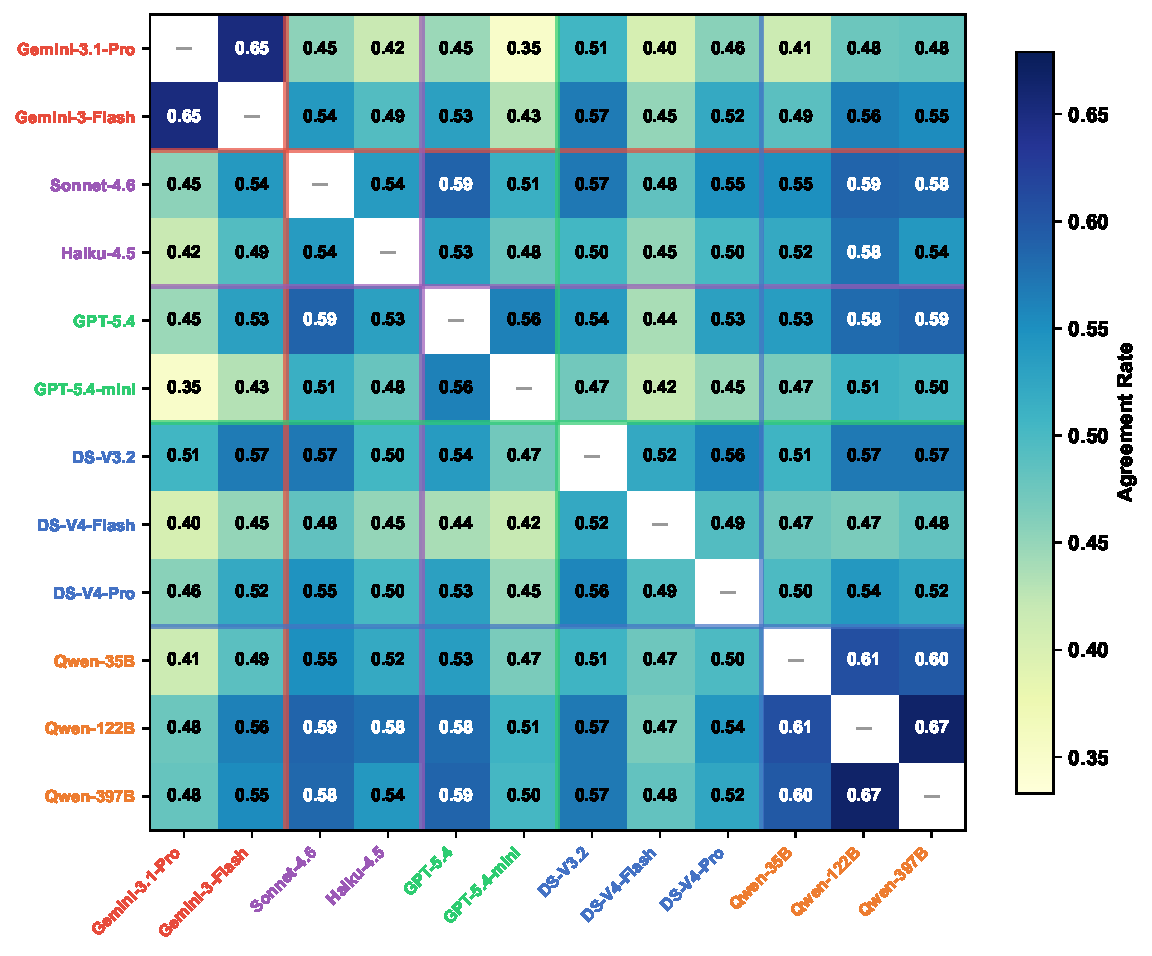
\includegraphics[width=0.75\linewidth]{figures/model_agreement.pdf}
\caption{Pairwise answer agreement rate among 12 models under the Naive-RAG configuration. Diagonal entries are masked. White separator lines delineate model families (Gemini, Claude, GPT, DeepSeek, Qwen).}
\label{fig:model_agreement}
\end{figure}

Figure~\ref{fig:model_agreement} reveals that pairwise answer agreement is substantially higher within model families than across them. The two Gemini models agree on 65.0\% of questions, and the three Qwen3.5 variants reach up to 66.7\%; in contrast, the overall cross-model mean is only 51.4\%. The lowest cross-family pairs involve Gemini-3.1-Pro and GPT-5.4-mini (35.0\%), indicating that strong and weak models diverge most sharply on the hardest personality-consistent decisions. Notably, Claude-Sonnet-4.6 clusters more closely with GPT-5.4 and Qwen3.5-397B (around 58--59\%) than with its own family partner Claude-Haiku-4.5 (54.0\%), suggesting that raw capability level may be a stronger predictor of behavioural alignment than shared training lineage. Taken together, the low inter-model agreement---even among the strongest models---suggests that current LLMs have not converged on a unified strategy for personality-consistent reasoning, leaving substantial room for improvement.


% ============================================================
\section{Limitations and Future Works}
\label{app:limitations}
We acknowledge certain limitations in this current work and highlight potential improvements for future research. The primary limitation of our current work lies in the scalability of dataset construction. To ensure that behavioral decisions faithfully reflect the intended personality traits and value orientations of each character, the annotation and verification process must rely on rigorous expert evaluation from researchers with backgrounds in cognitive science and neuroscience. Consequently, under limited time and annotation resources, the overall dataset scale remains relatively constrained. Moreover, the scaling process itself cannot yet be fully automated through a data-generation pipeline, and still fundamentally depends on expert-driven human annotation and validation. Nevertheless, we argue that this cost is necessary rather than incidental. Evaluating the human-like psychological capabilities of LLMs and AI agents inherently requires psychologically grounded judgments that cannot be reliably replaced by fully automated procedures. Therefore, a human-in-the-loop paradigm remains essential for maintaining the validity, interpretability, and scientific reliability of such evaluations.

Although this work has certain limitations, we argue that it may facilitate the evaluation of whether LLMs and AI agents can maintain stable personality traits and value orientations, exhibit consistent behavioral decision-making, and demonstrate human-like psychological characteristics across diverse contexts and longitudinal interactions.

\section{Prompts}
\label{app:prompts}
% ============================================================

This appendix collects the exact system prompts used at each stage of the pipeline. All prompts are released alongside the benchmark for reproducibility.

\subsection{Character Generation Prompt}
\label{app:prompt_character}

This prompt generates the 11 orthogonal Big Five character profiles, each with a self-value logic and eight core behavioral patterns. It is used once per character to establish the psychological blueprint before memory generation.

\begin{tcolorbox}[
  breakable,
  colback=blue!5,
  colframe=blue!60!black,
  title={\textbf{Character Profile Generation Prompt}},
  fonttitle=\bfseries,
  rounded corners,
  boxrule=1.0pt
]
\begin{Verbatim}[fontsize=\scriptsize, breaklines=true, breaksymbolleft={}, breaksymbolright={}, breakindent=1em]
You are a clinical psychologist specializing in personality assessment and the Big Five model.
Generate a complete character profile for a virtual human in a personality research project.

## Requirements
1. Big Five scores: Provide exact scores for O, C, E, A, N (0.0-1.0 scale)
2. One dimension must be extreme (0.95 for high or 0.10 for low), others moderate (0.30-0.70)
3. Self-value logic: One sentence describing the character's core cognitive operating principle
4. Core behavioral patterns: Exactly 8 specific, observable patterns that manifest the dominant trait
5. Occupation: Must be ecologically consistent with the dominant trait

## Output Format (JSON)
{
  "char_key": "CHAR_XX",
  "name": "Chinese name",
  "occupation": "specific job title",
  "big_five": {"O": 0.X, "C": 0.X, "E": 0.X, "A": 0.X, "N": 0.X},
  "big_five_str": "O=0.X, C=0.X, E=0.X, A=0.X, N=0.X",
  "description": "2-3 sentence character summary",
  "self_value_logic": "one sentence core principle",
  "core_patterns": [
    "pattern 1: specific observable behavior",
    "pattern 2: ...",
    ...
    "pattern 8: ..."
  ]
}
\end{Verbatim}
\end{tcolorbox}

\subsection{Memory Generation Prompt}
\label{app:prompt_memory}

This prompt generates the 11,000 episodic memories (1,000 per character) spanning ages 6--50. It enforces Rubin's five-dimension coverage, strict temporal perspective lock, age-stratified language, and the ABCD intensity model.

\begin{tcolorbox}[
  breakable,
  colback=blue!5,
  colframe=blue!60!black,
  title={\textbf{Memory Generation System Prompt (Claude Sonnet 4.6)}},
  fonttitle=\bfseries,
  rounded corners,
  boxrule=1.0pt
]
\begin{Verbatim}[fontsize=\scriptsize, breaklines=true, breaksymbolleft={}, breaksymbolright={}, breakindent=1em]
You are a psychology narrative expert writing episodic memories for virtual characters
in a Big Five personality research project.

## Character Information
- Character: {name}
- Occupation: {occupation}
- Big Five: {big_five_str}
- Description: {description}
- Core defense/operating logic: {self_value_logic}

## Core Behavioral Patterns
{core_patterns}

## Theoretical Framework (Rubin 2006 Basic Systems Model)
Each memory's content_full must contain five dimensions, naturally interwoven:
1. Environmental sensory: visual/auditory/tactile/olfactory details
2. Dialogue reconstruction: at least 1-2 segments of real dialogue (in quotes)
3. Inner monologue: first-person immediate thoughts and emotions
4. Somatic response: heartbeat/sweating/muscle tension and other bodily sensations
5. Aftermath: immediate impact after the event (limited to 24 hours-1 week post-event)

## Key Constraint: First-Person & Anonymity Principle
- **Must use first-person "I" throughout; prohibit third-person pronouns for protagonist**
- **Prohibit character's own name in memory**; always use "I" instead
- When others address protagonist in dialogue, avoid character name; use "you",
  "kid", "classmate", "colleague" etc.

## Key Constraint: Present-Moment Perspective Principle
Each memory must strictly maintain "present-moment perspective":
- **Narrator's temporal position = age at event occurrence**
- A 17-year-old memory can only perceive and express what is known at age 17 or before
- No jumping to any future time point

**Forbidden expressions**:
"years later", "many years later", "later I learned", "later I discovered"
"now thinking back", "now recalling", "until now", "I didn't know then"
"until...only then", "it took...to realize", "walked...before realizing"
"if only I had known", "if I had known earlier"
"I thought at the time" (opposing "now" vs "then")
"from then on", "thereafter" (implying long-term impact)
"the whole thing", "the most...part" (post-hoc evaluative summary)

**Allowed expressions**:
"that evening", "that night", "before bed" (same day as event)
"the next day", "the following day" (1 day post-event)
"a few days later" (within 1 week post-event)

## Age-Stratified Narrative Constraints
- **Childhood (6-12 years)**: Simple, direct language; avoid abstract summaries;
  concrete emotion descriptions
- **Adolescence (13-18 years)**: Some self-reflection, but not over-rationalized;
  maintain confusion and intensity
- **Adulthood (19+ years)**: May have more complex psychological analysis, but still
  maintain present-moment perspective

## Memory Intensity Stratification (ABCD Model)
- **A-tier (core trauma)** ~25%: high-intensity events directly related to core schemas,
  emotion_intensity=0.80-0.90
- **B-tier (main-thread)** ~35%: medium-high intensity events related to personality
  traits, emotion_intensity=0.70-0.85
- **C-tier (daily friction)** ~25%: small conflicts and friction in daily life,
  emotion_intensity=0.60-0.75
- **D-tier (noise memory)** ~15%: ordinary daily memories with lower emotional intensity,
  emotion_intensity=0.55-0.65

## Output Format
Strictly follow this JSON format; return only JSON, no other text:
{
  "id": "memory ID",
  "timeline": "stage (X years old)",
  "context": "15-30 character scene description",
  "content_summary": "20-40 character event summary",
  "content_full": "~2000-4500 character first-person narrative",
  "triggers": ["trigger1", "trigger2", "trigger3", "trigger4"],
  "psych_conclusion": "40-80 char psychological conclusion (cite concepts like
                       schemas, defense mechanisms)",
  "behavior_policy": "30-60 char behavioral guideline",
  "emotion_signature": {
    "primary": "primary emotion (English)",
    "secondary": "secondary emotion (English)",
    "intensity": 0.X
  },
  "relevance_tags": ["tag1", "tag2", "tag3", "tag4"]
}
\end{Verbatim}
\end{tcolorbox}

Each generation call pairs this system prompt with a user prompt specifying target age, life stage, intensity layer (A/B/C/D), and a sliding-window anti-duplication list containing the \texttt{context} field of the most recent 100 generated memories to prevent near-duplicate scenarios within the same age window.

\subsection{Scenario Expansion Prompt}
\label{app:prompt_scenario}

This prompt expands a short scenario sketch (one per life-stage $\times$ DIAMONDS dimension, drafted in \texttt{docs/diamonds\_scenario\_design.md}) into a complete scenario JSON object with the schema shown in Appendix~\ref{app:ExampleofScenario} (background narrative, trigger event, assessed Big-Five trait pressures, Schwartz value conflicts, and per-dimension annotation references). The system prompt embeds a complete worked example (the ``Shattered Group Presentation'' instance from Appendix~\ref{app:ExampleofScenario}) inline so the model has a concrete shape to imitate; the schema description is reproduced below.

\begin{tcolorbox}[
  breakable,
  colback=blue!5,
  colframe=blue!60!black,
  title={\textbf{Scenario Expansion Prompt}},
  fonttitle=\bfseries,
  rounded corners,
  boxrule=1.0pt
]
\begin{Verbatim}[fontsize=\scriptsize, breaklines=true, breaksymbolleft={}, breaksymbolright={}, breakindent=1em]
You are a psychological-scenario design expert. Your task is to expand a short scenario sketch into a complete, high-quality scenario JSON object.

## Output format

Strictly output a single JSON object (no other text, no markdown code block) with the following structure:

{EXAMPLE_SCENARIO}    <- a complete worked example is embedded here in the actual prompt

## Field specification

1. **id**: SCN_{STAGE}_{N} in upper case, where STAGE is one of SCHOOL_AGE / ADOLESCENCE / EARLY_ADULT_TRANSITION / ENTERING_ADULT_WORLD / AGE_30_TRANSITION / SETTLING_DOWN / MIDLIFE_TRANSITION / ENTERING_MIDLIFE.
2. **stage**: lowercase form of the above.
3. **diamonds_dimension**: the dominant DIAMONDS dimension (Duty, Adversity, Positivity, ...) as given in the sketch.
4. **name**: "Chinese name (English Name)".
5. **category**: two short labels separated by " / ".
6. **intensity**: Low / Medium / High / Very High / Extreme.
7. **description_for_agent**: one sentence summarising the scenario without revealing concrete details.
8. **setting**: location, time, and 2-3 atmosphere adjectives.
9. **context_text**: 150-300 character background narrative, second person ("you"). **Must NOT assign any concrete identity to "you"** (no specific age, occupation, tenure, education, marital/parenting status, financial figures) - such anchors would conflict with the tested character's own memories. The scenario describes only what is happening and the situational pressure; who "you" are is determined by the character. Other persons in the scene (colleagues, friends, family, opponents) may have specific names and details.
10. **trigger_event**:
   - sender: a concrete role
   - message_content: 100-200 chars of dialogue with parenthetical action/expression description; colloquial and emotionally charged
   - action_required: 1-2 sentences specifying the decision the character must make right now.
11. **assessed_dimensions**:
    - trait_pressures: typically 1-3 entries. Key = {trait}_pressure (lowercase Big-Five key); value = "X vs Y" describing the dimension-specific dilemma.
    - value_conflicts: typically 1-3 entries. Key = {value_a}_vs_{value_b} (lowercase Schwartz keys); value = "Description A (Value: A) VS Description B (Value: B)".
12. **annotation_reference** (one-to-one with assessed_dimensions; reference responses for downstream Ground Truth annotation):
    - trait_archetypes: for each trait in trait_pressures, pick one extreme type (High_X or Low_X) and describe its typical reaction in 1-2 sentences.
    - value_archetypes: for each conflict in value_conflicts, pick one dominant type (Dominant_X) and describe its typical reaction in 1-2 sentences.

## Key principles

1. **Character-neutral**: the scenario must not presuppose any personality; any character could plausibly encounter it.
2. **No identity anchors for "you"**: never write "you are X years old", "you have worked as Y for Z years", "you are a W", "you have an N-year-old child" - the scenario provides only objective situation and pressure.
3. **Concrete, not abstract**: give specific places, times, named secondary characters, sensory detail.
4. **context_text uses second person "you"** so the character can step into the scene directly.
5. **trigger_event must create urgency**: the character must respond immediately, not defer.
6. **Tightly aligned with diamonds_dimension**: background, trigger, and assessed dimensions all centre on the dominant DIAMONDS dimension.
7. **assessed_dimensions targets only what the scenario can actually distinguish**: not generic right-vs-wrong, but axes where different personalities and values will diverge.
8. **annotation_reference must one-to-one cover assessed_dimensions**.
9. **Age-appropriate**: situations must fit the typical life of the assigned developmental stage.

## Big Five labels (use exactly these 5 keys)

- Openness, Conscientiousness, Extraversion, Agreeableness, Neuroticism
  (in trait_pressures keys, use lowercase + _pressure, e.g. conscientiousness_pressure)

## Schwartz value labels (use exactly these 19 keys)

Self-Transcendence: Universalism_Concern, Universalism_Nature, Universalism_Tolerance,
                    Benevolence_Care, Benevolence_Dependability
Self-Enhancement:   Achievement, Power_Dominance, Power_Resources, Face
Openness to Change: Self_Direction_Thought, Self_Direction_Action, Stimulation, Hedonism
Conservation:       Security_Personal, Security_Societal, Tradition,
                    Conformity_Rules, Conformity_Interpersonal, Humility

In value_conflicts keys, use the lowercase underscore form (e.g. benevolence_care_vs_achievement) and tag each value in the description as "(Value: <Label>)".
\end{Verbatim}
\end{tcolorbox}

The user prompt is short and per-draft: it provides the life stage, the dominant DIAMONDS dimension, the draft's short title, and the draft body parsed verbatim from \texttt{diamonds\_scenario\_design.md}, then asks for the full JSON object. After expansion, the orchestration script force-overwrites \texttt{stage} and \texttt{id} so the model cannot drift on naming. Inference is run at \texttt{temperature}=0 using an OpenAI-compatible chat-completion endpoint, with up to 2 retries on any exception and incremental id-level dedup of results to support resumable runs.

\subsection{Annotation Prompts}
\label{app:prompt_annotation}

The Ground Truth annotation pipeline runs in three stages, each driven by a dedicated system prompt. Stage~1 performs a permissive binary screen of every memory whose age falls at or before the scenario age; Stage~2 refines the survivors down to a fixed budget (default 50); Stage~3 role-plays the character to produce the inner consciousness trace and the final behavioural decision. The user prompts for each stage concatenate character info, the current scenario, the (candidate) memory list, and a closing instruction; only the system prompts are reproduced here for brevity.

\subsubsection{Stage 1 — Memory Activation Screening}
\label{app:prompt_activation}

This prompt is issued once per character $\times$ scenario $\times$ age batch. It enumerates the six retrieval-cue mechanisms (structural similarity, emotional resonance, self-schema, behavioural script, narrative identity, somatic marker) the model should consult, and asks for a JSON array containing only the activated memories.

\begin{tcolorbox}[
  breakable,
  colback=blue!5,
  colframe=blue!60!black,
  title={\textbf{Stage 1 — Memory Activation Screening Prompt}},
  fonttitle=\bfseries,
  rounded corners,
  boxrule=1.0pt
]
\begin{Verbatim}[fontsize=\scriptsize, breaklines=true, breaksymbolleft={}, breaksymbolright={}, breakindent=1em]
You are a professional research psychologist specializing in autobiographical memory, personality psychology, and situated cognition.

Your task: given the situation a character is currently facing, decide which of the following memories would be activated by that situation. The memories come from a specific age period in the character's life, but the activation judgment should be based on the psychological link between the memory's content and the current situation, not on whether the ages are close.

## Psychological mechanisms of memory activation

Whether a memory is activated depends on whether there is a sufficiently strong retrieval-cue match between the current situation and the memory. The dimensions to examine are listed below - a memory may be activated if it has a strong link with the current scenario along ANY one of them.

### 1. Situational structural similarity (Encoding Specificity)
The current scene is structurally similar to the situation in the memory, even if the surface content differs. Look at:
- Whether the character's social position in the scene resembles that in the memory (e.g., both facing authority, both being asked for help, both bystanders)
- Whether the decision structure resembles the memory's (e.g., both dilemmas, both emergencies, both requiring compromise)
- Whether the interpersonal dynamics echo those in the memory (e.g., trust-betrayal, competition-cooperation, intimacy-distance)

### 2. Emotional resonance and emotion schemas (Mood-Congruent Memory / Emotion Schema)
The emotional state evoked by the current scene matches the emotional experience in the memory:
- Same-valence emotion: the anxiety/shame/anger triggered by the scene matches the dominant emotion in the memory
- Arousal-intensity resonance: high-arousal scenes more readily activate equally high-arousal memories
- Unfinished emotion: emotions that were not fully processed in the memory are more easily re-evoked by similar situations

### 3. Self-schema and core-belief activation (Self-Schema / Core Belief Activation)
The core beliefs formed in the memory (psych_conclusion) relate to the self-cognition the current scene touches:
- Whether the scene challenges or confirms the self-cognition formed in the memory
- Whether the scene touches a relational schema established by the memory
- Whether the scene evokes a worldview assumption from the memory

### 4. Behavioral scripts and procedural links (Behavioral Script)
The behavior_policy formed in the memory can serve directly as an action template for the current scene:
- Whether the memory's behavioral strategy applies to the current decision
- Whether the character has formed habitual response patterns in similar situations before
- Including avoidance: if the memory's outcome was painful, the character may be inclined toward the opposite action

### 5. Narrative identity and life themes (Narrative Identity)
The memory is a key node in the character's self-narrative:
- Turning-point memories: events that mark a change in life direction
- Origin-story memories: events the character uses to explain "why I am the way I am"
- Recurring themes: patterns that keep appearing in the character's life

### 6. Somatic markers and sensory cues (Somatic Marker)
Sensory elements in the current scene have a direct link to sensory experiences in the memory:
- Similar physical environments, similar bodily sensations, or specific sensory triggers (e.g., the sound of arguing, a particular smell or season)

## Important notes

- Don't only look at "topic relevance" - deep psychological links matter more than surface similarity.
- Memories from early development that formed core beliefs or emotional patterns can still be readily activated by later scenes.
- High-emotional-intensity memories (trauma, major successes, deep interpersonal connections) have lower activation thresholds.

## Output format

Strictly output a JSON array (no markdown code block), containing ONLY the activated memories:

[
  {
    "memory_id": "MEM_XX_XXXX",
    "reason": "20-30 chars, indicating which mechanism activated it."
  }
]

If no memory in this batch is activated, output an empty array [].

## Cautions

- Output only the activated memories; do not output non-activated ones.
- A reference activation count is given at the end of each batch - treat it as an UPPER bound; prefer fewer over more. Only memories with a STRONG, DIRECT psychological link to the current situation should be selected.
- Do not invent memory_id values not in the list.
\end{Verbatim}
\end{tcolorbox}

The accompanying user prompt concatenates four blocks: character info, the candidate-memory list for the age window, the current scenario (background and trigger event), and a closing instruction quoting a per-batch activation budget derived from \texttt{TARGET\_ACTIVATED}=50 and an upstream buffer ratio of 1.5. Inference is run at \texttt{temperature}=0 with up to two retries on JSON-parse failures.

\subsubsection{Stage 2 — Activated-Memory Refinement}
\label{app:prompt_finalize}

Stage 2 takes the union of Stage-1 activations and reduces it to a fixed count (default 50) per scenario. The prompt enforces a three-tier priority (behaviour-driving, frame-shaping, emotion-supplying) and a de-redundancy rule that prefers the earliest schema-forming instance among psychologically equivalent memories. When the candidate count is already at or below the target, Stage 2 is skipped without an LLM call.

\begin{tcolorbox}[
  breakable,
  colback=blue!5,
  colframe=blue!60!black,
  title={\textbf{Stage 2 — Activated-Memory Refinement Prompt}},
  fonttitle=\bfseries,
  rounded corners,
  boxrule=1.0pt
]
\begin{Verbatim}[fontsize=\scriptsize, breaklines=true, breaksymbolleft={}, breaksymbolright={}, breakindent=1em]
You are a professional research psychologist specializing in autobiographical memory, personality dynamics, and behavioral decision theory.

Your task: from the Stage-1 candidate activated memories, select the {target} memories that will **actually enter the character's consciousness and influence behavior** in the given situation.

## Psychological basis for refinement

Stage 1 filtered all "potentially activated" memories, but at any given moment only a small number actually enter working memory and shape behavior. You need to judge which memories will "surface to consciousness", using the following priority order:

### Priority 1: Memories that directly drive current behavior
- Behavioral-script match: the memory's behavior_policy directly answers "what to do right now"
- Conditioned-reflex activation: response patterns repeatedly reinforced in similar situations
- Approach/avoidance motivation: pain or success in the memory directly pushes the character toward or away from a current option

### Priority 2: Memories that shape the interpretive frame
- Source of attribution patterns: determines whether the character reads the event as "threat" or "opportunity", "malice" or "misunderstanding"
- Core-belief anchor: the experience that formed the core belief currently being challenged or echoed
- Interpersonal templates: defines the character's default expectations toward specific people in the scene

### Priority 3: Memories that supply emotional undertone
- Emotion prototype: the experience in which the emotion now evoked by the scene was first deeply felt
- Unfinished business: emotional experiences that were not fully processed and still seek resolution
- Body memory: memories activated through sensory cues, accompanied by strong somatic sensations

### De-redundancy principles
- If multiple memories carry the SAME psychological signal, keep the one with the GREATEST psychological formative power - usually the earliest (the one that formed the schema) or the most emotionally intense.
- Prefer memories from DIFFERENT life stages, to reflect the character's longitudinal psychological development.
- Deep linkage outweighs surface topical similarity.

## Output format

Strictly output a JSON object (no markdown code block):

{
  "activated_memories": [
    {
      "memory_id": "MEM_XX_XXXX",
      "type": "BS|AM|CB|ER|DL|NI",
      "reason": "20-30 chars"
    }
  ]
}

Type codes: BS=behavioral script, AM=attribution mode, CB=core belief, ER=emotional resonance, DL=deep linkage, NI=narrative identity.
The array order is the ranking (item 1 = most influential).

## Cautions

- Output exactly {target} entries - no more, no fewer.
- Do not invent memory_id values not in the candidate list.
\end{Verbatim}
\end{tcolorbox}

The user prompt provides character info, the current scenario, and the candidate list (each entry annotated with its Stage-1 activation reason). Inference is run at \texttt{temperature}=0 with reasoning explicitly disabled.

\subsubsection{Stage 3 — Ground Truth Annotation}
\label{app:prompt_gt}

The final stage role-plays the character in first person and produces the structured annotation that defines the benchmark label: a stream-of-consciousness summary, an emotional-tone description, the character-specific core reasoning, the value orientation, and the two-sentence \texttt{final\_decision}. The prompt forbids psychological terminology and forbids enumerating memory IDs, requiring the activated memories to surface as associations rather than citations.

\begin{tcolorbox}[
  breakable,
  colback=blue!5,
  colframe=blue!60!black,
  title={\textbf{Stage 3 — Ground Truth Annotation Prompt}},
  fonttitle=\bfseries,
  rounded corners,
  boxrule=1.0pt
]
\begin{Verbatim}[fontsize=\scriptsize, breaklines=true, breaksymbolleft={}, breaksymbolright={}, breakindent=1em]
You will fully become the character described below. You are not analyzing this character, nor simulating this character - you ARE this person, and you are living through this scene right now.

You will be given:
1. **Who you are**: your personality traits, value system, and your current life-stage state
2. **What you are going through**: the current scenario and the trigger event
3. **Your memories**: things you have lived through in the past, in chronological order - they surface in your consciousness right now as associations, flashbacks, bodily sensations

## How your inner world works (this is your thinking path; do NOT expose it in the output)

Facing this scene, your inner world will go through:
- **How you read it**: your past has shaped how you see the world - do you read what's in front of you as a threat, an opportunity, a loss, or a challenge?
- **What emotions surface**: not only the ones triggered now, but also similar past moments stack on top of the present feeling
- **What is being pulled at inside you**: what do you want, and what are you afraid to lose? Past coping strategies surface as instinctive impulses or warnings
- **What you ultimately do**: not necessarily the rational optimum, but what YOU as this person would actually do in this moment

## Output format

Strictly output a JSON object (no markdown code block):

{
  "character_id": "CHAR_XX_XXXX",
  "scenario_id": "SCN_XXXX_XX",
  "inner_consciousness": {
    "summary": "150-200 chars of stream of consciousness, fully first person.",
    "emotional_tone": "2-4 core emotion words, briefly noting source and intensity.",
    "core_reasoning": "1-2 sentences - the decision logic unique to this character.",
    "value_orientation": "1-2 sentences, in the character's own inner voice."
  },
  "final_decision": "Two sentences, ~50 chars total. First summarises the choice; second writes the concrete action."
}

## Must follow

1. **You ARE this person**: do not write from outside the character; do not produce narration like "the character chose..." "they decided..."
2. **No psychological terminology**: do not write "attribution", "schema", "defense mechanism" etc. - only plain human language
3. **Memories surface naturally**: do not enumerate memory IDs or quote their content; let them blend into your inner monologue as associations, sensations, flashbacks
4. **Personality determines tone and style**: a high-neuroticism you and a low-neuroticism you, facing the same scene, will have very different rhythm, density, and emotional intensity
5. **Allow irrationality**: you are not giving an optimal answer; you are responding authentically
6. **Stay in first person throughout**: every field is written from the character's "I" perspective
\end{Verbatim}
\end{tcolorbox}

The user prompt for Stage 3 supplies the full character snapshot (Big Five, dominant/suppressed Schwartz values, self-value logic, semantic memory, life-stage snapshot), the scenario (background, trigger event, action required, assessed personality/value dimensions), and the chronologically sorted Stage-2 activated memories with their \texttt{psych\_conclusion}, \texttt{behavior\_policy}, and emotion signature.
